% ---------------------------------------------------------------------------
% VT analysis report — LaTeX template
%
% Rendered by analysis.py with Jinja2. Values are inserted with VAR placeholders
% and logic with BLOCK statements. Edit the layout and wording freely; keep the
% placeholders. Figures are vector PDFs in report/figures/.
% ---------------------------------------------------------------------------
\documentclass[11pt,a4paper]{article}

% Computer Modern, LaTeX's default typeface (classic OT1 encoding, Type 1 fonts)
\usepackage[utf8]{inputenc}
\usepackage[a4paper,margin=2.4cm,top=2.3cm,bottom=2.6cm]{geometry}
\usepackage{microtype}
\usepackage{graphicx}
\usepackage{booktabs}
\usepackage{tabularx}
\usepackage{array}
\usepackage[table]{xcolor}
\usepackage{caption}
\usepackage{enumitem}
\usepackage{titlesec}
\usepackage{fancyhdr}
\usepackage{amsmath}
\usepackage{amssymb}
\usepackage{float}
\usepackage[round]{natbib}
\usepackage{needspace}
\usepackage[hidelinks]{hyperref}

\definecolor{ink}{HTML}{121211}
\definecolor{muted}{HTML}{6E6D68}
\definecolor{accent}{HTML}{1F5FAD}
\definecolor{rule}{HTML}{C9C8C0}

\graphicspath{{figures/}}
\setlength{\parindent}{0pt}
\setlength{\parskip}{0.55em}
\renewcommand{\arraystretch}{1.18}
\setlength{\aboverulesep}{0.25ex}
\setlength{\belowrulesep}{0.4ex}

\titleformat{\section}{\Large\bfseries\color{ink}}{\thesection}{0.7em}{}
\titleformat{\subsection}{\large\bfseries\color{ink}}{\thesubsection}{0.6em}{}
\titlespacing*{\section}{0pt}{1.6em}{0.6em}
\titlespacing*{\subsection}{0pt}{1.2em}{0.35em}
\newcommand{\keep}[1]{\Needspace{#1\baselineskip}}

\captionsetup{font=small,labelfont=bf,labelsep=period,justification=raggedright,singlelinecheck=false,skip=4pt}
\captionsetup[table]{position=top}

\renewcommand{\labelitemi}{$\bullet$}  % keeps every glyph in Type 1 Computer Modern
\newcommand{\note}[1]{{\footnotesize\color{muted}#1\par}}
\newcolumntype{R}{>{\raggedleft\arraybackslash}X}
\newcolumntype{L}{>{\raggedright\arraybackslash}X}

\pagestyle{fancy}
\fancyhf{}
\renewcommand{\headrulewidth}{0pt}
\fancyfoot[L]{\footnotesize\color{muted} Vanguard Total World Stock ETF (VT) --- Price analysis since inception}
\fancyfoot[R]{\footnotesize\color{muted} \thepage}

\hypersetup{pdftitle={VT -- Price analysis since inception}, pdfauthor={\VAR{author}}}

\begin{document}

% ---------------------------------------------------------------- Title
\thispagestyle{fancy}
{%
{\footnotesize\color{muted}\MakeUppercase{Market data report} $\cdot$ \VAR{generated}}\par\vspace{0.6em}
{\fontsize{22}{26}\selectfont\bfseries\color{ink} Vanguard Total World Stock ETF (VT)\par}\vspace{0.3em}
{\large\color{muted} Price analysis since inception, \VAR{first_date} -- \VAR{last_date}\par}\vspace{0.2em}
{\small\color{muted} \VAR{author} $\cdot$ \VAR{n_days} trading days $\cdot$ Yahoo Finance data, validated against Vanguard\par}
}
\vspace{0.4em}

\section*{Summary}

\begin{table}[H]
\footnotesize
\begin{tabularx}{\linewidth}{L r}
\toprule
\textbf{Metric} & \textbf{Value} \\
\midrule
Price at inception $\rightarrow$ latest price & USD \VAR{px0} $\rightarrow$ \VAR{px1} \\
Cumulative return (price / total return) & \VAR{cum_px} / \VAR{cum_tr} \\
Annualised return (price / total return) & \VAR{cagr_px} / \VAR{cagr_tr} \\
Annualised total return in CHF & \VAR{cagr_chf} \\
Annualised volatility (monthly returns; daily $\times\sqrt{252}$ in brackets) & \VAR{vol} (\VAR{vol_d}) \\
Sharpe ratio, 95\% confidence interval (average risk-free rate \VAR{rf_mean}) & \VAR{sharpe} \VAR{sharpe_ci} \\
Sortino ratio & \VAR{sortino} \\
Maximum drawdown (total return) & \VAR{mdd} (trough on \VAR{mdd_date}) \\
Calmar ratio & \VAR{calmar} \\
Kelly exposure with borrowing spread, in-sample (block-bootstrap 95\% interval) & \VAR{L_s} \VAR{L_ci} \\
Probability of loss over 1 / 5 / 10 years: historical windows & \VAR{ploss_emp} \\
Probability of loss over 1 / 5 / 10 years: block bootstrap & \VAR{ploss_boot} \\
\bottomrule
\end{tabularx}
\end{table}

\subsection*{Key findings}
\begin{itemize}[leftmargin=1.2em,itemsep=0.3em,topsep=0.2em]
\BLOCK{for t in takeaways}
  \item \VAR{t}
\BLOCK{endfor}
\end{itemize}

\clearpage
% ---------------------------------------------------------------- 1
\section{Return and risk}

\begin{figure}[H]
\centering
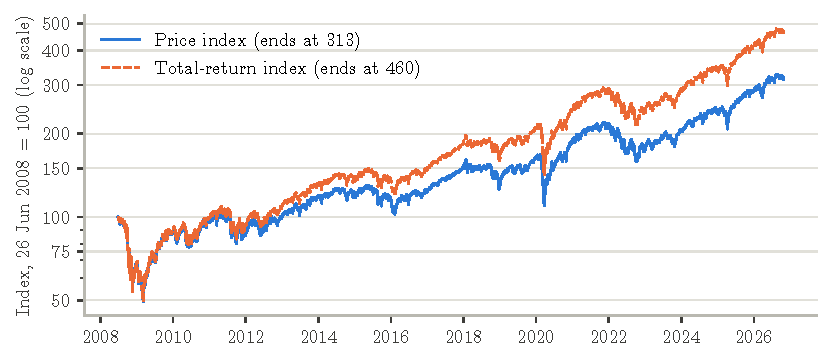
\includegraphics[width=\linewidth]{price.pdf}
\caption{Price index and total-return index (dividends reinvested), both rebased to 100 at inception, log scale. The gap between the two lines is the cumulative contribution of reinvested dividends; equal slopes represent equal percentage returns.}
\end{figure}

\keep{16}\subsection{Calendar-year returns}
\begin{figure}[H]
\centering
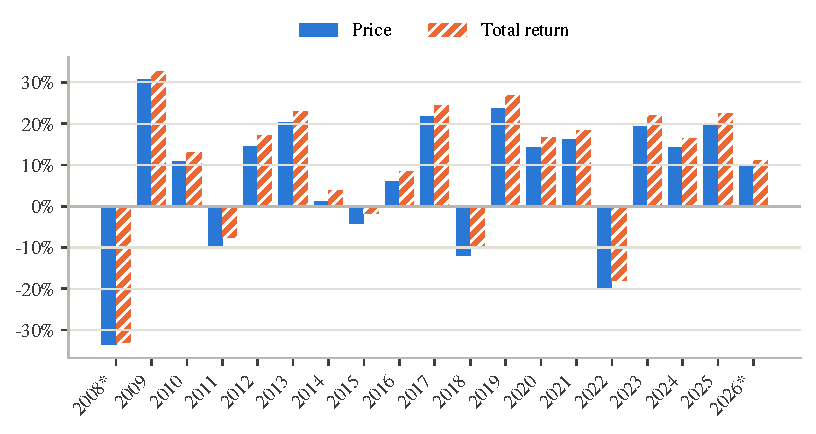
\includegraphics[width=\linewidth]{annual.pdf}
\caption{Calendar-year returns, price and total return. * Partial years.}
\end{figure}
\note{\VAR{annual_note}}

\keep{16}\subsection{Volatility}
\begin{figure}[H]
\centering
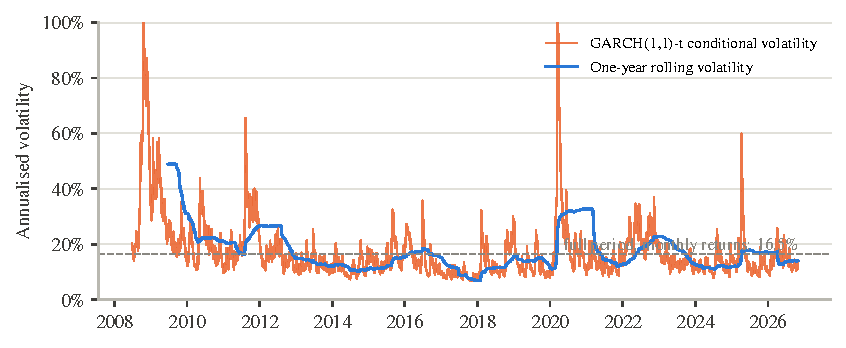
\includegraphics[width=\linewidth]{volatility.pdf}
\caption{Annualised daily volatility: exponentially weighted moving average (RiskMetrics, $\lambda = 0.94$) and GARCH(1,1)-$t$ conditional volatility with parameters estimated on the full sample. Dashed line: full-period volatility on the same daily basis.}
\end{figure}

\begin{table}[H]
\small
\caption{Annualised volatility by sampling frequency (non-overlapping total returns).}
\begin{tabularx}{\linewidth}{L r r}
\toprule
\textbf{Frequency} & \textbf{Observations} & \textbf{Annualised volatility} \\
\midrule
\BLOCK{for r in vol_freq_rows}
\VAR{r[0]} & \VAR{r[1]} & \VAR{r[2]} \\
\BLOCK{endfor}
\bottomrule
\end{tabularx}
\end{table}
\VAR{vol_text}

\keep{16}\subsection{Drawdowns}
\begin{figure}[H]
\centering
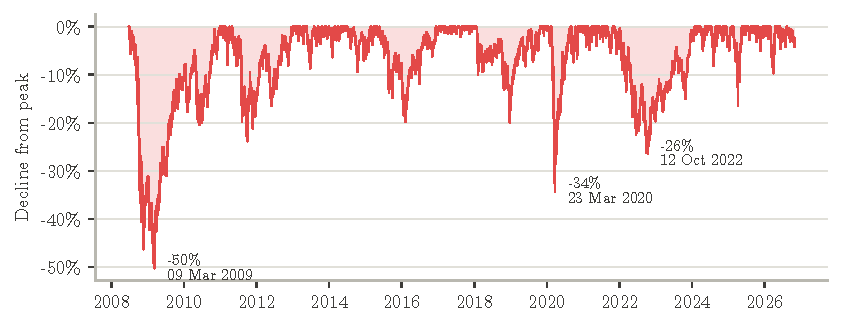
\includegraphics[width=\linewidth]{drawdown.pdf}
\caption{Decline of the total-return index from its previous peak.}
\end{figure}

\begin{table}[H]
\small
\caption{Five largest drawdowns (total return).}
\begin{tabularx}{\linewidth}{l l l R R R}
\toprule
\textbf{Peak} & \textbf{Trough} & \textbf{Recovery} & \textbf{Drawdown} & \textbf{Decline (days)} & \textbf{Recovery (days)} \\
\midrule
\BLOCK{for r in dd_rows}
\VAR{r[0]} & \VAR{r[1]} & \VAR{r[2]} & \VAR{r[3]} & \VAR{r[4]} & \VAR{r[5]} \\
\BLOCK{endfor}
\bottomrule
\end{tabularx}
\end{table}
\note{Lengths in trading days. Because VT was launched during the global financial crisis, the first peak is the launch date itself.}

\keep{16}\subsection{Risk-adjusted performance by sub-period}
\begin{table}[H]
\small
\caption{Return and risk by sub-period (total return; volatility and ratios from monthly returns).}
\begin{tabularx}{\linewidth}{L r r r c r r}
\toprule
\textbf{Period} & \textbf{Ann.\ return} & \textbf{Volatility} & \textbf{Sharpe} & \textbf{95\% CI} & \textbf{Sortino} & \textbf{Max.\ DD} \\
\midrule
\BLOCK{for r in sub_rows}
\BLOCK{if loop.last}\midrule{}\BLOCK{endif}
\VAR{r[0]} & \VAR{r[1]} & \VAR{r[2]} & \VAR{r[3]} & \VAR{r[4]} & \VAR{r[5]} & \VAR{r[6]} \\
\BLOCK{endfor}
\bottomrule
\end{tabularx}
\end{table}
\note{Excess returns over the 13-week US T-bill (\texttt{\^{}IRX}). Sharpe: mean excess return divided by its volatility. Sortino: mean excess return divided by the downside deviation of excess returns. Confidence intervals for the Sharpe ratio use the standard error of \citet{mertens2002} and \citet{opdyke2007}, which accounts for skewness and kurtosis.}

\VAR{sub_text}

% ---------------------------------------------------------------- 2
\keep{24}
\section{Distribution, volatility dynamics and Value at Risk}

\begin{figure}[H]
\centering
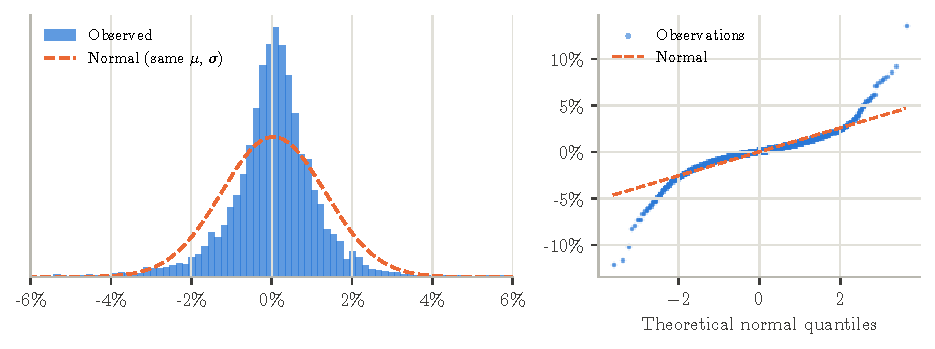
\includegraphics[width=\linewidth]{distribution.pdf}
\caption{Daily total returns: histogram against a normal density with the same mean and variance (left), and normal Q--Q plot (right).}
\end{figure}

\begin{table}[H]
\small
\caption{Descriptive statistics of daily returns.}
\begin{tabularx}{\linewidth}{L r r}
\toprule
\textbf{Statistic} & \textbf{Value} & \textbf{Normal benchmark} \\
\midrule
Mean / standard deviation & \VAR{mu} / \VAR{sd} & -- \\
Skewness & \VAR{skew} & 0 \\
Kurtosis & \VAR{kurt} & 3 \\
Jarque--Bera statistic & \VAR{jb} & -- \\
Days beyond $\pm 4$ standard deviations & \VAR{beyond4} & \VAR{expected4} expected \\
Worst day & \VAR{worst} & -- \\
Best day & \VAR{best} & -- \\
\bottomrule
\end{tabularx}
\end{table}
\VAR{dist_text}

\keep{16}\subsection{Volatility clustering and GARCH estimates}
\begin{figure}[H]
\centering
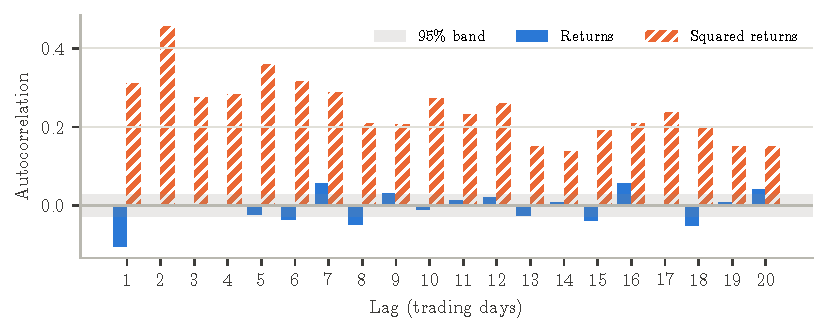
\includegraphics[width=\linewidth]{acf.pdf}
\caption{Autocorrelation of daily log returns and squared log returns, lags 1 to 20, with the 95\% band under independence.}
\end{figure}
\VAR{acf_text}

\begin{table}[H]
\small
\caption{GARCH(1,1) with standardised Student-$t$ innovations, maximum-likelihood estimates (full sample).}
\begin{tabularx}{\linewidth}{L r r}
\toprule
\textbf{Parameter} & \textbf{Estimate} & \textbf{Standard error} \\
\midrule
\BLOCK{for r in garch_rows}
\VAR{r[0]} & \VAR{r[1]} & \VAR{r[2]} \\
\BLOCK{endfor}
\bottomrule
\end{tabularx}
\end{table}
\note{Standard errors from the inverse of the numerical Hessian of the log-likelihood.}

\VAR{garch_text}

\keep{16}\subsection{Value at Risk: out-of-sample backtest}
\begin{figure}[H]
\centering
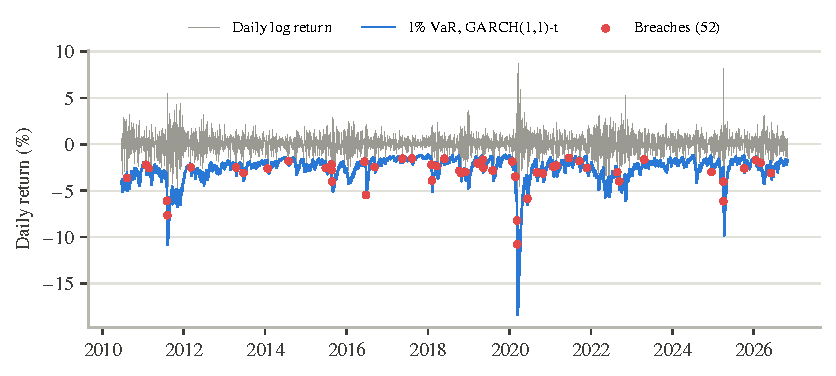
\includegraphics[width=\linewidth]{var_backtest.pdf}
\caption{Daily returns and one-day 1\% VaR forecast by the GARCH(1,1)-$t$ model; red dots mark breaches.}
\end{figure}

\begin{table}[H]
\small
\caption{Backtest of one-day VaR forecasts (\VAR{n_bt} days from \VAR{bt_start}); $p$-values of the coverage tests.}
\begin{tabularx}{\linewidth}{l L r r r r r}
\toprule
\textbf{Level} & \textbf{Method} & \textbf{Breach rate} & \textbf{Breaches / expected} & \textbf{Kupiec} & \textbf{Christoff.} & \textbf{CC} \\
\midrule
\BLOCK{for r in bt_rows}
\VAR{r[0]} & \VAR{r[1]} & \VAR{r[2]} & \VAR{r[3]} & \VAR{r[4]} & \VAR{r[5]} & \VAR{r[6]} \\
\BLOCK{endfor}
\bottomrule
\end{tabularx}
\end{table}
\note{\VAR{bt_note}}

\VAR{bt_text}

\begin{table}[H]
\small
\caption{GARCH(1,1)-$t$ VaR backtest under three treatments of the conditional mean.}
\begin{tabularx}{\linewidth}{l L r r r r r}
\toprule
\textbf{Level} & \textbf{Mean specification} & \textbf{Breach rate} & \textbf{Breaches / exp.} & \textbf{Kupiec} & \textbf{Christoff.} & \textbf{CC} \\
\midrule
\BLOCK{for r in mean_rows}
\VAR{r[0]} & \VAR{r[1]} & \VAR{r[2]} & \VAR{r[3]} & \VAR{r[4]} & \VAR{r[5]} & \VAR{r[6]} \\
\BLOCK{endfor}
\bottomrule
\end{tabularx}
\end{table}
\VAR{mean_text}

\keep{16}\subsection{Variance forecasts: out-of-sample comparison}
\begin{table}[H]
\small
\caption{Out-of-sample variance forecasts over the backtest period. Lower losses are better; Diebold--Mariano test of QLIKE against EWMA.}
\begin{tabularx}{\linewidth}{l L r r r r r}
\toprule
\textbf{Horizon} & \textbf{Model} & \textbf{QLIKE} & \textbf{MSE} & \textbf{Rank} & \textbf{DM stat.} & \textbf{$p$-value} \\
\midrule
\BLOCK{for r in fe_rows}
\BLOCK{if loop.index == 4}\midrule{}\BLOCK{endif}
\VAR{r[0]} & \VAR{r[1]} & \VAR{r[2]} & \VAR{r[3]} & \VAR{r[4]} & \VAR{r[5]} & \VAR{r[6]} \\
\BLOCK{endfor}
\bottomrule
\end{tabularx}
\end{table}
\note{Variances in squared percent. Proxy: squared daily return (1 day) and realised variance, the sum of the next 21 squared daily returns (21 days). GARCH: zero-mean model re-estimated each year, multi-step forecasts from its persistence and long-run variance; EWMA and historical variance are held flat over the horizon. Rank by QLIKE. Diebold--Mariano statistics use a Newey--West variance (5 and 25 lags); a negative value favours the model over EWMA.}

\VAR{fe_text}

% ---------------------------------------------------------------- 3
\keep{24}
\section{Market efficiency}

\subsection{First-order autocorrelation}
\begin{table}[H]
\small
\caption{First-order autocorrelation of log returns.}
\begin{tabularx}{\linewidth}{L r r r r r r}
\toprule
\textbf{Frequency} & \textbf{Obs.} & \textbf{$\hat\rho_1$} & \textbf{Naive $t$} & \textbf{Robust $z$} & \textbf{$p$-value} & \textbf{Holm $p$} \\
\midrule
\BLOCK{for r in ac_rows}
\VAR{r[0]} & \VAR{r[1]} & \VAR{r[2]} & \VAR{r[3]} & \VAR{r[4]} & \VAR{r[5]} & \VAR{r[6]} \\
\BLOCK{endfor}
\bottomrule
\end{tabularx}
\end{table}
\note{Naive $t = \hat\rho_1\sqrt{n}$ assumes independent, identically distributed returns. The robust $z$ uses the heteroskedasticity-consistent standard error $\sqrt{\sum e_t^2 e_{t-1}^2}\,/\sum e_t^2$; $p$-values refer to the robust statistic. Holm: adjusted for the \VAR{n_family|string} tests of this section.}

\VAR{ac_text}

\keep{16}\subsection{Variance ratio test}
Under the random-walk hypothesis, the variance of $q$-period returns is $q$ times the one-period variance, so
\[
VR(q) = \frac{\operatorname{Var}\left(r_t + r_{t-1} + \dots + r_{t-q+1}\right)}{q \,\operatorname{Var}(r_t)} = 1 .
\]
A ratio below 1 signals mean reversion, a ratio above 1 persistence. Following \citet{lo1988}, the statistic $z^*(q)$ is robust to heteroskedasticity, which is essential given the volatility clustering documented above.

\begin{table}[H]
\small
\caption{Lo--MacKinlay variance ratio test on daily log total returns.}
\begin{tabularx}{\linewidth}{l r r r r R}
\toprule
\textbf{Horizon $q$ (days)} & \textbf{$VR(q)$} & \textbf{$z^*(q)$} & \textbf{$p$-value} & \textbf{Holm $p$} & \textbf{Conclusion (Holm)} \\
\midrule
\BLOCK{for r in vr_rows}
\VAR{r[0]} & \VAR{r[1]} & \VAR{r[2]} & \VAR{r[3]} & \VAR{r[4]} & \VAR{r[5]} \\
\BLOCK{endfor}
\bottomrule
\end{tabularx}
\end{table}

\keep{16}\subsection{Calendar effects}
\begin{figure}[H]
\centering
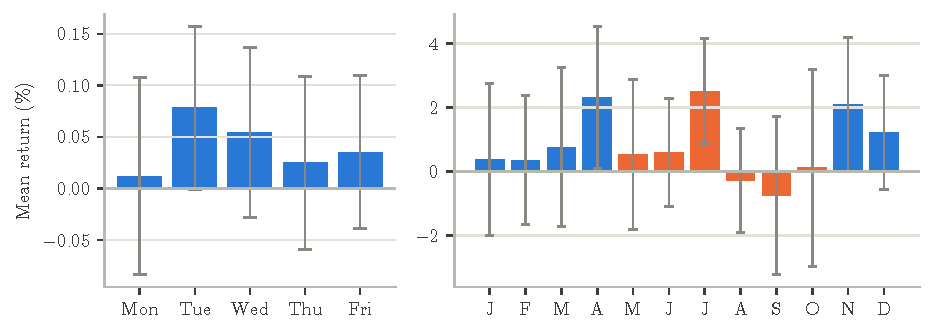
\includegraphics[width=\linewidth]{calendar.pdf}
\caption{Mean daily return by weekday (left) and mean monthly return by calendar month (right), with 95\% confidence intervals. May to October in orange.}
\end{figure}

\begin{table}[H]
\small
\caption{Tests of calendar effects.}
\begin{tabularx}{\linewidth}{L r r r}
\toprule
\textbf{Test} & \textbf{Result} & \textbf{$p$-value} & \textbf{Holm $p$} \\
\midrule
Equal mean returns across weekdays (ANOVA) & \VAR{cal_day} & \VAR{p_day} & \VAR{h_day} \\
January effect: January vs other months (Welch) & \VAR{cal_jan} & \VAR{p_jan} & \VAR{h_jan} \\
``Sell in May'': Nov--Apr vs May--Oct, per half-year (\VAR{n_halves}) & \VAR{cal_sim} & \VAR{p_sim} & \VAR{h_sim} \\
\bottomrule
\end{tabularx}
\end{table}
\note{\VAR{cal_note}}

\keep{12}\subsection{Multiple testing}
\VAR{mt_text}

\keep{16}\subsection{Moving-average timing rules}
\begin{figure}[H]
\centering
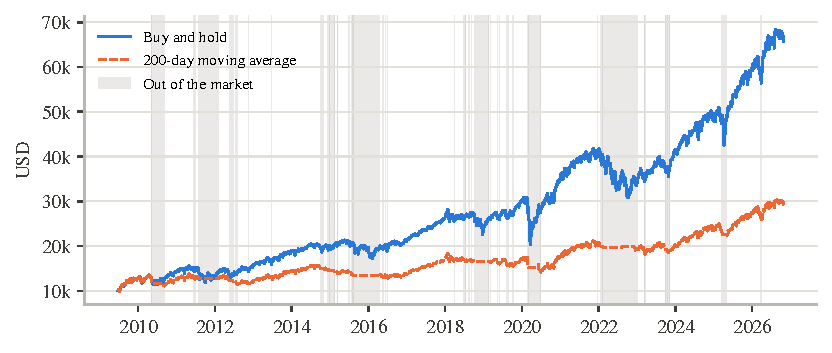
\includegraphics[width=\linewidth]{ma200.pdf}
\caption{Growth of USD 10{,}000 from \VAR{ma_start}: buy and hold vs the 200-day moving-average rule. Shaded areas: rule out of the market.}
\end{figure}

\begin{table}[H]
\small
\caption{Buy and hold vs 200-day moving average (Sharpe ratio with 95\% confidence interval).}
\begin{tabularx}{\linewidth}{L r r}
\toprule
 & \textbf{Buy and hold} & \textbf{200-day moving average} \\
\midrule
Annualised return & \VAR{ma[0][0]} & \VAR{ma[0][1]} \\
Volatility & \VAR{ma[1][0]} & \VAR{ma[1][1]} \\
Sharpe ratio & \VAR{ma[2][0]} & \VAR{ma[2][1]} \\
Maximum drawdown & \VAR{ma[3][0]} & \VAR{ma[3][1]} \\
Final value of USD 10{,}000 & \VAR{ma[4][0]} & \VAR{ma[4][1]} \\
\bottomrule
\end{tabularx}
\end{table}

\begin{table}[H]
\small
\caption{Sensitivity to the moving-average window and to execution (common period). Volatility, Sharpe and drawdown refer to the main execution.}
\begin{tabularx}{\linewidth}{L r r r r r r r}
\toprule
\textbf{Window} & \textbf{Ann.\ return} & \textbf{Delayed} & \textbf{Volatility} & \textbf{Sharpe} & \textbf{Max.\ DD} & \textbf{Switches} & \textbf{Invested} \\
\midrule
\BLOCK{for r in ma_sens_rows}
\BLOCK{if loop.last}\midrule{}\BLOCK{endif}
\VAR{r[0]} & \VAR{r[1]} & \VAR{r[2]} & \VAR{r[3]} & \VAR{r[4]} & \VAR{r[5]} & \VAR{r[6]} & \VAR{r[7]} \\
\BLOCK{endfor}
\bottomrule
\end{tabularx}
\end{table}
\note{\VAR{ma_note}}

\VAR{ma_text}

% ---------------------------------------------------------------- 4
\keep{24}
\section{Holding period and investor behaviour}

\subsection{Rolling returns and the probability of loss}
\begin{figure}[H]
\centering
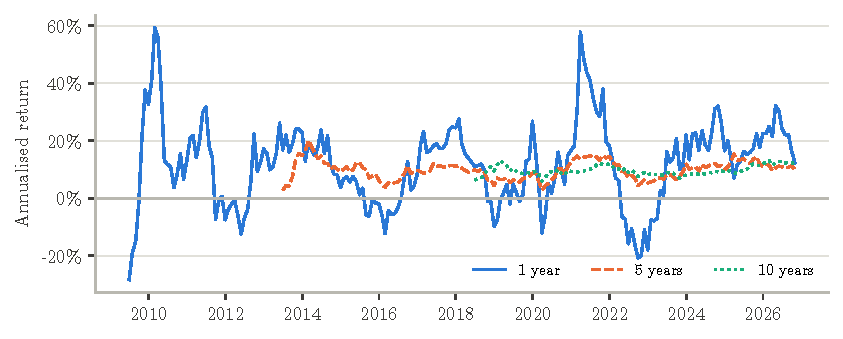
\includegraphics[width=\linewidth]{rolling.pdf}
\caption{Annualised total return over rolling 1-, 5- and 10-year windows, by end of window.}
\end{figure}

\begin{table}[H]
\small
\caption{Rolling returns (overlapping monthly windows, annualised) and bootstrap probability of loss.}
\begin{tabularx}{\linewidth}{l r r r R r r}
\toprule
\textbf{Horizon} & \textbf{Windows} & \textbf{P(loss)} & \textbf{Bootstrap} & \textbf{Worst (window end)} & \textbf{Median} & \textbf{Best} \\
\midrule
\BLOCK{for r in roll_rows}
\VAR{r[0]} & \VAR{r[1]} & \VAR{r[2]} & \VAR{r[3]} & \VAR{r[4]} & \VAR{r[5]} & \VAR{r[6]} \\
\BLOCK{endfor}
\bottomrule
\end{tabularx}
\end{table}
\VAR{roll_text}

\begin{table}[H]
\footnotesize
\begin{minipage}[t]{0.48\linewidth}
\caption{Bootstrap probability of loss by mean block length (months).}
\begin{tabularx}{\linewidth}{L r r r}
\toprule
\textbf{Block} & \textbf{1 year} & \textbf{5 years} & \textbf{10 years} \\
\midrule
\BLOCK{for r in block_rows}
\VAR{r[0]} & \VAR{r[1]} & \VAR{r[2]} & \VAR{r[3]} \\
\BLOCK{endfor}
\bottomrule
\end{tabularx}
\end{minipage}\hfill
\begin{minipage}[t]{0.48\linewidth}
\caption{Normal i.i.d. model: probability of loss with the mean at its estimate and at the ends of its 95\% interval.}
\begin{tabularx}{\linewidth}{L r r r}
\toprule
\textbf{Horizon} & \textbf{Estimate} & \textbf{High $\mu$} & \textbf{Low $\mu$} \\
\midrule
\BLOCK{for r in param_rows}
\VAR{r[0]} & \VAR{r[1]} & \VAR{r[2]} & \VAR{r[3]} \\
\BLOCK{endfor}
\bottomrule
\end{tabularx}
\end{minipage}
\end{table}

\keep{16}\subsection{Sensitivity to the starting date}
\begin{figure}[H]
\centering
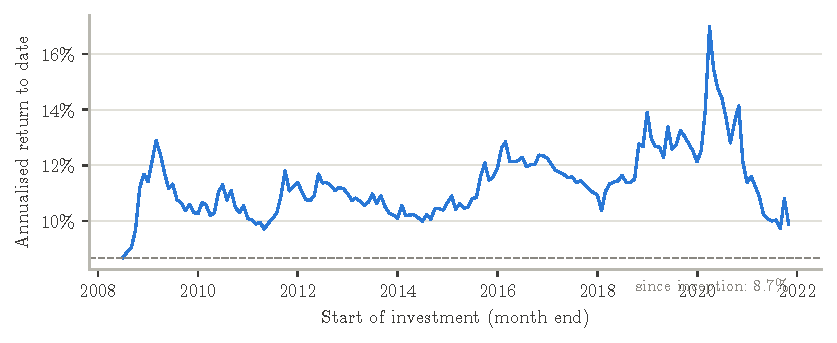
\includegraphics[width=\linewidth]{start_date.pdf}
\caption{Annualised total return from each month end to the latest close (starting points with at least five years of history).}
\end{figure}
\VAR{start_text}

\keep{16}\subsection{The cost of missing the best days}
\begin{figure}[H]
\centering
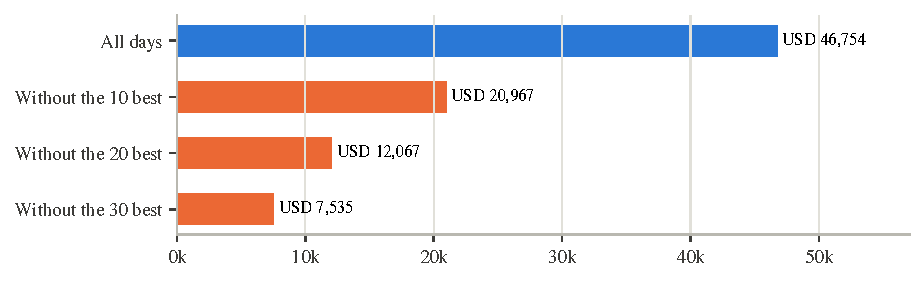
\includegraphics[width=\linewidth]{best_days.pdf}
\caption{Final value of USD 10{,}000 invested at inception, with and without the best trading days.}
\end{figure}
\VAR{best_text}

\keep{16}\subsection{Monthly savings plan and lump-sum investing}
\begin{figure}[H]
\centering
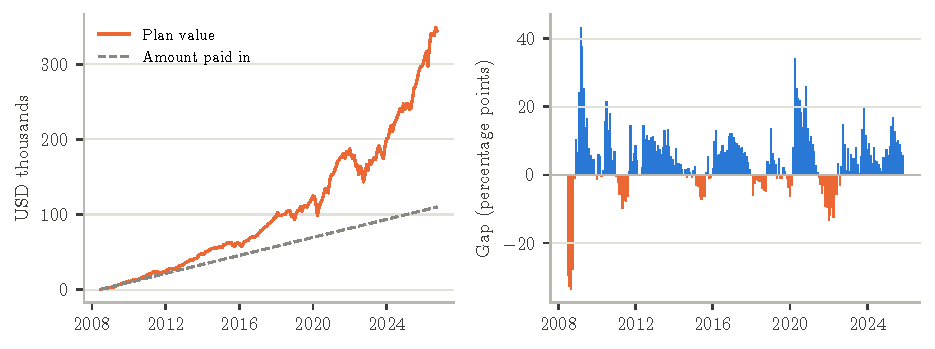
\includegraphics[width=\linewidth]{savings.pdf}
\caption{Left: value of a USD \VAR{contribution} monthly plan vs amount paid in. Right: lump sum minus 12-month averaging, value gap after 12 months, by starting month.}
\end{figure}
\VAR{plan_text}

% ---------------------------------------------------------------- 4.5 Kelly
\keep{20}\subsection{Optimal leverage, Kelly criterion and volatility drag}
\label{sec:kelly}
Can leverage raise the long-run compounded growth of an investment in VT, and by how much? This subsection derives the growth-optimal exposure, estimates it, tests it out of sample and separates the effects that make leveraged compounding differ from a simple multiple of the fund's return. The aim is not to show that leverage pays, but to identify the assumptions under which it maximises expected growth and to show how fragile that optimum is.

\paragraph{Framework.} Suppose the fund's value follows a geometric Brownian motion with arithmetic expected return $\mu$ and volatility $\sigma$, and an investor holds a constant exposure $L$ to it, rebalanced continuously, with the rest in cash at the rate $r_f$ ($L<1$) or financed by borrowing ($L>1$). $L=1$ is the unleveraged fund, $L=0.5$ a 50\% exposure and $L=2$ a 200\% exposure. If borrowing costs $r_f$, wealth $W$ grows at the expected logarithmic rate
\[
g(L) = \frac{1}{\mathrm{d}t}\,\mathbb{E}\left[\mathrm{d}\log W_t\right] = r_f + L(\mu - r_f) - \tfrac{1}{2}L^2\sigma^2 .
\]
The arithmetic expected return of the portfolio, $r_f + L(\mu - r_f)$, rises linearly with $L$, but the expected log growth carries the quadratic penalty $\tfrac{1}{2}L^2\sigma^2$. Since $g'(L) = (\mu - r_f) - L\sigma^2$ and $g''(L) = -\sigma^2 < 0$, the function is strictly concave and maximised at the Kelly exposure \citep{kelly1956,breiman1961,merton1969}
\[
L^* = \frac{\mu - r_f}{\sigma^2}, \qquad g(L^*) = r_f + \frac{(\mu - r_f)^2}{2\sigma^2}.
\]
$\mu$ is an arithmetic mean: substituting the historical CAGR, which is already a log-growth rate net of the drag $\tfrac12\sigma^2$, would count the drag twice.

\paragraph{Borrowing costs.} A retail investor borrows above the rate earned on cash. With a lending rate $r_l$ and a borrowing rate $r_b > r_l$, the growth rate is piecewise:
\[
g(L) = \begin{cases} r_l + L(\mu - r_l) - \tfrac12 L^2\sigma^2, & 0 \le L \le 1,\\[2pt] r_b + L(\mu - r_b) - \tfrac12 L^2\sigma^2, & L > 1. \end{cases}
\]
It remains concave, with a kink at $L=1$. The optimum is $(\mu - r_l)/\sigma^2$ if that is below one, $(\mu - r_b)/\sigma^2$ if that is above one, and exactly one otherwise: leverage is worth taking only if the marginal expected return exceeds the marginal borrowing cost by more than the marginal variance penalty. Margin rates are not available in the data, so the borrowing rate is set to the T-bill yield plus a spread of \VAR{k_spread} a year, comparable to the lower end of retail margin rates; Table~\ref{tab:ksens} reports spreads from 0 to 3\%. The T-bill yield itself is a lending rate, not an observable margin rate.

\paragraph{Simulation.} The strategies are simulated on daily simple total returns $r_t$ from the adjusted prices, so dividends are included and fund expenses, already in the price, are not charged again. For an exposure $L$ decided at the close of day $t-1$,
\[
W_t = W_{t-1}\left(1 + R_{p,t} - c_t\right), \qquad R_{p,t} = \begin{cases} L r_t + (1-L)\, r_{l,t}, & 0\le L\le1,\\ L r_t - (L-1)\, r_{b,t}, & L>1, \end{cases}
\]
where $r_{l,t}$ is the T-bill yield known at the previous close divided by 252, $r_{b,t} = r_{l,t} + \text{spread}/252$, and $c_t$ is a cost of \VAR{k_cost}\,bp per unit of exposure traded when the position is rebalanced to its target at the close. With $L=1$ nothing is traded and the simulation reproduces buy-and-hold exactly. If $1 + R_{p,t} - c_t \le 0$, the strategy is insolvent and its wealth stays at zero. Five numerical checks are run on every update: $L=1$ reproduces the fund's total-return path, $L=0$ reproduces the cash account, the closed-form $L^*$ matches the numerical maximum of $g$, the exact decomposition below reconciles with simulated wealth to machine precision, and wealth cannot recover after insolvency.

\begin{table}[H]
\small
\caption{Kelly inputs and leverage estimates (full sample).}
\label{tab:kelly}
\begin{tabularx}{\linewidth}{L r}
\toprule
\textbf{Input} & \textbf{Estimate} \\
\midrule
\BLOCK{for r in k_param_rows}
\VAR{r[0]} & \VAR{r[1]} \\
\BLOCK{endfor}
\midrule
\textbf{Exposure} & \\
\BLOCK{for r in k_L_rows}
\VAR{r[0]} (\VAR{r[2]}) & \VAR{r[1]} \\
\BLOCK{endfor}
\bottomrule
\end{tabularx}
\end{table}
\VAR{k_est_text}

\begin{figure}[H]
\centering
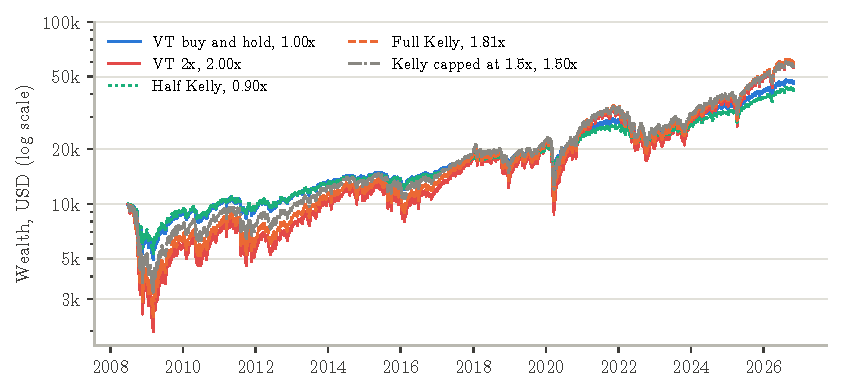
\includegraphics[width=\linewidth]{kelly_wealth.pdf}
\caption{Historical simulation, not a forecast: growth of USD 10{,}000 under constant exposures rebalanced daily, borrowing at the T-bill rate plus \VAR{k_spread}, \VAR{k_cost}\,bp rebalancing costs. Kelly exposures are estimated on the full sample (hindsight).}
\end{figure}

\begin{table}[H]
\small
\caption{Constant-exposure strategies, full sample, daily rebalancing, borrowing spread \VAR{k_spread}. Volatility and Sharpe ratio from monthly returns, as in Section~1.}
\label{tab:kstrat}
\begin{tabularx}{\linewidth}{L r r r r r r r}
\toprule
\textbf{Strategy} & \textbf{$L$} & \textbf{CAGR} & \textbf{Vol.} & \textbf{Sharpe} & \textbf{Max.\ DD} & \textbf{Final (USD)} & \textbf{Margin days} \\
\midrule
\BLOCK{for r in k_strat_rows}
\VAR{r[0]} & \VAR{r[1]} & \VAR{r[2]} & \VAR{r[3]} & \VAR{r[4]} & \VAR{r[5]} & \VAR{r[6]} & \VAR{r[7]} \\
\BLOCK{endfor}
\bottomrule
\end{tabularx}
\end{table}
\VAR{k_strat_text}

\VAR{k_margin_text}

\paragraph{Volatility drag and the compounding gap.} Three different effects separate a leveraged position from ``$L$ times the fund'', in addition to trading costs. To isolate the effect of leverage on compounding, compare the frictionless daily-reset position financed at a rate $b_t$ with the geometrically scaled reference $\log W^{\text{ref}}_T = L\sum_t \log(1+r_t) - (L-1)\sum_t\log(1+b_t)$. The difference is
\begin{align*}
D_T(L) &= \sum_{t=1}^{T}\Big[\log\big(1 + L r_t - (L-1) b_t\big) - L\log(1+r_t) + (L-1)\log(1+b_t)\Big] \\
&\approx -\tfrac12 L(L-1)\sum_{t=1}^{T}(r_t - b_t)^2 ,
\end{align*}
where the approximation uses second-order expansions of the logarithms and requires every wealth factor to be positive \citep{cheng2009,avellaneda2010}. The gap is zero for $L=0$ and $L=1$, negative for $L>1$, and grows with realised variance and with $L(L-1)$.

\begin{table}[H]
\small
\caption{Exact decomposition of annualised log growth, full sample, spread \VAR{k_spread}, \VAR{k_cost}\,bp costs. Components add up to the total.}
\label{tab:kdecomp}
\setlength{\tabcolsep}{4pt}
\begin{tabularx}{\linewidth}{l R R R R R R}
\toprule
\textbf{$L$} & \textbf{$L\times$ log growth of VT} & \textbf{T-bill financing} & \textbf{Borrowing spread} & \textbf{Compoun\-ding gap} & \textbf{Trading costs} & \textbf{Total log growth} \\
\midrule
\BLOCK{for r in k_decomp_rows}
\VAR{r[0]} & \VAR{r[1]} & \VAR{r[2]} & \VAR{r[3]} & \VAR{r[4]} & \VAR{r[5]} & \VAR{r[6]} \\
\BLOCK{endfor}
\bottomrule
\end{tabularx}
\end{table}
\VAR{k_drag_text}

\begin{figure}[H]
\centering
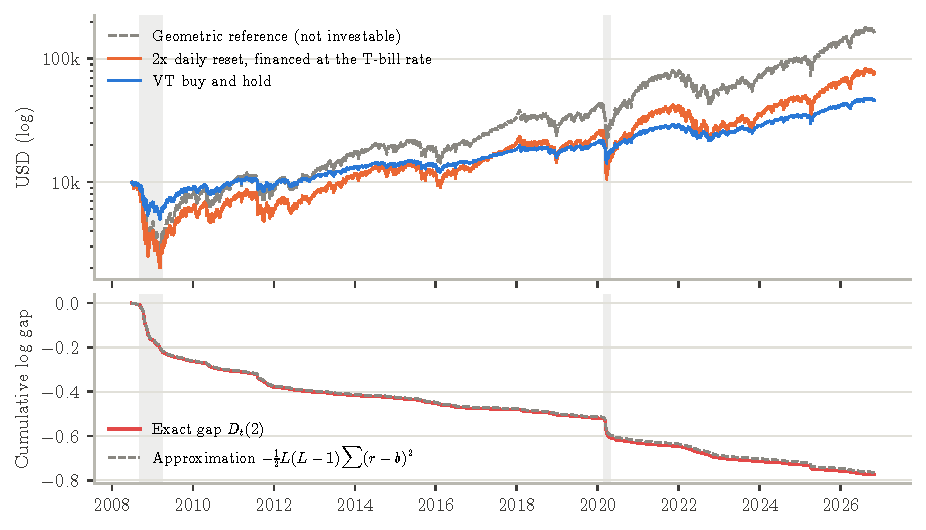
\includegraphics[width=\linewidth]{kelly_drag.pdf}
\caption{Historical simulation: a frictionless 2x daily-reset position financed at the T-bill rate, its geometrically scaled reference and VT (top); cumulative exact compounding gap and its approximation (bottom). Shaded: September 2008 to March 2009 and February to April 2020.}
\end{figure}
\VAR{k_path_text}

\paragraph{Growth as a function of leverage.} Figure~\ref{fig:kgrowth} plots the model growth curve and the growth actually realised by each constant exposure. The curves are concave: below the optimum, more leverage adds growth; beyond it, the quadratic penalty dominates and growth falls, turning negative around 4x. The realised curve follows the model closely because both use the same sample, which is precisely why its maximum is not a guide to the future. The shaded band shows how far the model curve moves when $\mu$ is set to either end of its 95\% confidence interval: the uncertainty grows with $L$, and at 2x the band is \VAR{k_band2} percentage points of annual growth wide.

\begin{figure}[H]
\centering
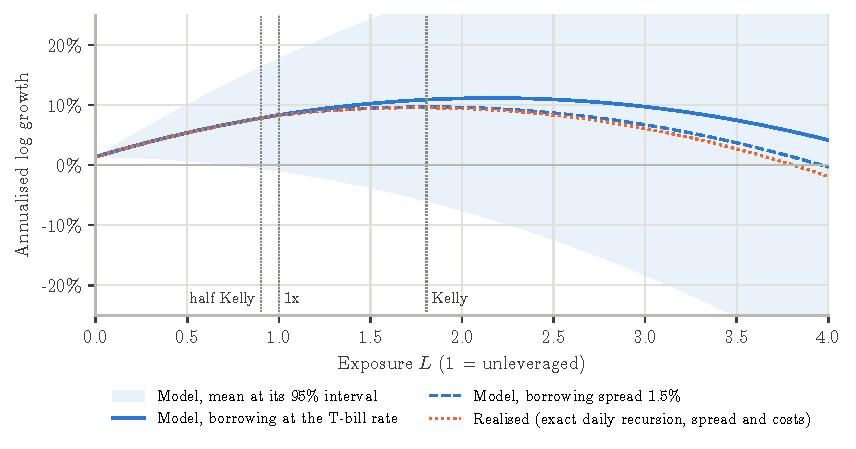
\includegraphics[width=\linewidth]{kelly_growth.pdf}
\caption{Model-implied expected log growth $g(L)$ (blue, with and without the borrowing spread; band: mean return at the ends of its 95\% interval) and realised log growth of the daily simulations (orange, in-sample). Vertical lines: 1x, half Kelly and Kelly with the spread.}
\label{fig:kgrowth}
\end{figure}

\paragraph{Estimation uncertainty.} \VAR{k_unc_text}

\begin{table}[H]
\small
\caption{Circular block bootstrap of the frictionless Kelly exposure (\VAR{n_boot} resamples of daily excess returns).}
\begin{tabularx}{\linewidth}{L r r r r}
\toprule
\textbf{Block length} & \textbf{Median} & \textbf{95\% interval} & \textbf{P($L^*<1$)} & \textbf{P($L^*>2$)} \\
\midrule
\BLOCK{for r in k_boot_rows}
\VAR{r[0]} & \VAR{r[1]} & \VAR{r[2]} & \VAR{r[3]} & \VAR{r[4]} \\
\BLOCK{endfor}
\bottomrule
\end{tabularx}
\end{table}

\begin{table}[H]
\small
\caption{Kelly exposure under alternative inputs, one input changed at a time (borrowing at the T-bill rate unless stated).}
\label{tab:ksens}
\begin{tabularx}{\linewidth}{l L r}
\toprule
\textbf{Input} & \textbf{Value} & \textbf{$L^*$} \\
\midrule
\BLOCK{for r in k_sens_rows}
\BLOCK{if loop.index > 1 and r[0] != loop.previtem[0]}\midrule{}\BLOCK{endif}
\VAR{r[0]} & \VAR{r[1]} & \VAR{r[2]} \\
\BLOCK{endfor}
\bottomrule
\end{tabularx}
\end{table}

\paragraph{Out-of-sample test.} \VAR{k_oos_text}

\begin{figure}[H]
\centering
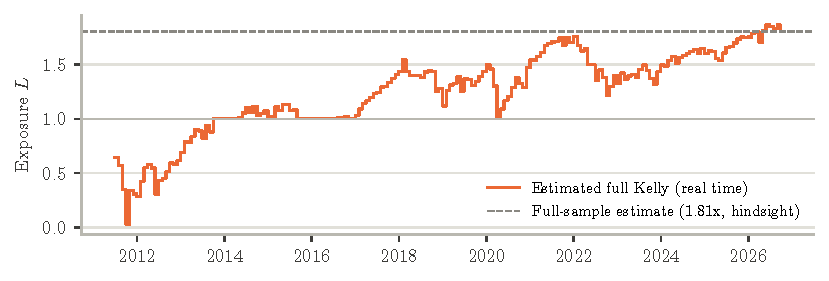
\includegraphics[width=\linewidth]{kelly_oos.pdf}
\caption{Kelly exposure estimated in real time at each month end (expanding window, borrowing spread \VAR{k_spread}), compared with the full-sample estimate available only in hindsight.}
\end{figure}

\begin{table}[H]
\small
\caption{Out-of-sample comparison from \VAR{oos_start} (common period, daily rebalancing, spread \VAR{k_spread}, \VAR{k_cost}\,bp costs).}
\label{tab:koos}
\begin{tabularx}{\linewidth}{L r r r r r r}
\toprule
\textbf{Strategy} & \textbf{$L$: mean (range)} & \textbf{CAGR} & \textbf{Vol.} & \textbf{Sharpe} & \textbf{Max.\ DD} & \textbf{Final (USD)} \\
\midrule
\BLOCK{for r in k_oos_rows}
\VAR{r[0]} & \VAR{r[1]} & \VAR{r[2]} & \VAR{r[3]} & \VAR{r[4]} & \VAR{r[5]} & \VAR{r[6]} \\
\BLOCK{endfor}
\bottomrule
\end{tabularx}
\end{table}

\paragraph{Interpretation.} Historical VT returns imply a growth-optimal exposure of about \VAR{L_s} with realistic borrowing costs, but this number is an in-sample artefact of one favourable eighteen-year path rather than a parameter that can be relied on. Its 95\% interval spans almost the whole range from no leverage to 4x, it moves by about one unit of leverage or more with plausible changes to the expected return, the variance or the period, and a real-time estimate would not have found it. The features documented earlier in this report work against aggressive leverage: fat tails and volatility clustering (Section~2) mean that losses arrive in bursts, exactly when the compounding gap widens and margin calls occur; the \VAR{mdd_1x} drawdown of 2008--2009 becomes \VAR{mdd_fk} at full Kelly and \VAR{mdd_2x} at 2x; and the confidence interval of the Sharpe ratio (Section~1) is the same uncertainty that makes $L^*$ unknowable. Because the growth curve is flat near its maximum and falls steeply beyond it, overestimating $L^*$ is far more costly than underestimating it. This asymmetry is the case for fractional Kelly \citep{thorp2006,maclean2011}: under the model, half Kelly keeps three quarters of the growth gain while halving the volatility\BLOCK{if half_below_one}, and at the point estimate it does not even require borrowing\BLOCK{endif}.

% ---------------------------------------------------------------- 5
\keep{24}
\section{A Swiss investor's perspective}
\begin{figure}[H]
\centering
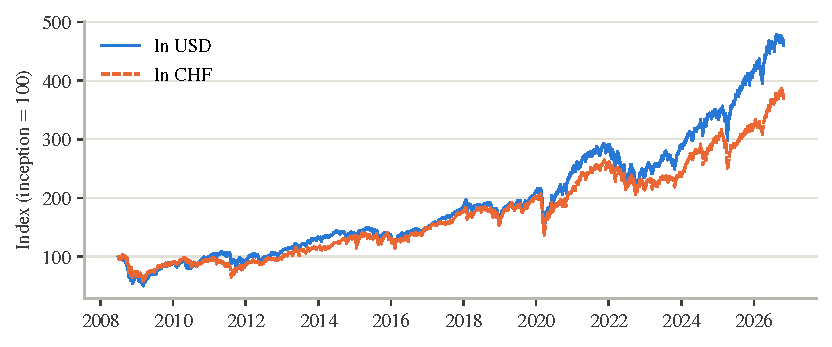
\includegraphics[width=\linewidth]{chf.pdf}
\caption{Total return in USD and in CHF, rebased to 100 at inception.}
\end{figure}

\begin{table}[H]
\small
\caption{VT in US dollars and in Swiss francs.}
\begin{tabularx}{\linewidth}{L r r}
\toprule
 & \textbf{In USD} & \textbf{In CHF} \\
\midrule
Annualised total return & \VAR{cagr_usd} & \VAR{cagr_chf} \\
Annualised volatility (monthly returns) & \VAR{vol} & \VAR{vol_chf} \\
USD/CHF over the period & -- & \VAR{fx_move} \\
Correlation of VT with USD/CHF (weekly / daily) & -- & \VAR{corr_w} / \VAR{corr_d} \\
\bottomrule
\end{tabularx}
\end{table}
\VAR{chf_text}

% ---------------------------------------------------------------- 6
\keep{24}
\section{Data validation}
\BLOCK{if val_available}
\begin{table}[H]
\small
\caption{Total returns from Yahoo adjusted prices vs Vanguard's published returns, to 30 September 2026.}
\begin{tabularx}{\linewidth}{L r r r r}
\toprule
\textbf{Period} & \textbf{Vanguard, market price} & \textbf{This report} & \textbf{Gap (pp)} & \textbf{Vanguard, NAV} \\
\midrule
\BLOCK{for r in val_rows}
\VAR{r[0]} & \VAR{r[1]} & \VAR{r[2]} & \VAR{r[3]} & \VAR{r[4]} \\
\BLOCK{endfor}
\bottomrule
\end{tabularx}
\end{table}
\note{Periods of one year or more are annualised. Source: Vanguard fact sheet F3141 (data as of 30 September 2026), stored in \texttt{data/reference/}.}
\BLOCK{endif}

\VAR{val_text}

% ---------------------------------------------------------------- 7
\keep{20}
\section{Limitations}
\begin{itemize}[leftmargin=1.2em,itemsep=0.3em,topsep=0.2em]
  \item \textbf{One asset, one period.} All results come from a single fund over eighteen years that include one global financial crisis, one pandemic crash and a long bull market. Estimates of mean returns and Sharpe ratios are imprecise over such horizons, as the confidence intervals show.
  \item \textbf{Start date.} VT was launched just before the 2008 crash, which depresses every ``since inception'' figure and works against timing rules that would have protected investors during that crash.
  \item \textbf{Data source.} Yahoo Finance is not an official source, and its adjusted prices can be revised retroactively. The validation against Vanguard covers a single reference date.
  \item \textbf{Market price vs NAV.} The analysis uses closing market prices. The daily autocorrelation may partly reflect gaps between the market price and the net asset value, which cannot be tested without daily NAV data.
  \item \textbf{Taxes and costs.} Returns are gross of investor-level taxes and trading costs (fund expenses are already reflected in the price). Dividends are assumed to be reinvested at the closing price on the ex-dividend date.
  \item \textbf{Leverage simulations.} Section~\ref{sec:kelly} assumes the target exposure is restored at each close at a small cost, ignores intraday moves, forced liquidations and taxes, and uses an assumed borrowing spread rather than observed margin rates. Its results are historical simulations, not achievable track records.
  \item \textbf{Model choices.} GARCH(1,1) with symmetric Student-$t$ errors does not capture the asymmetric response of volatility to losses (leverage effect) nor the skewness of large losses. Bootstrap results assume that the dependence structure of the past repeats.
\end{itemize}

% ---------------------------------------------------------------- 8
\keep{12}
\section{Conclusion}
The evidence describes a broadly diversified equity fund that has delivered the equity risk premium with the usual features of equity returns: fat tails, volatility that clusters and persists, and deep but temporary drawdowns.

Three statements about efficiency need to be kept apart. Statistically, the random walk is rejected only for a small negative daily autocorrelation; failing to reject it at longer horizons does not prove that prices are efficient, because the tests have limited power with eighteen years of data. In terms of predictability, the effect explains about \VAR{ac_r2} of the variance of daily returns and is concentrated in crises. Economically, none of the simple rules examined, moving averages or calendar strategies, created value after costs. The data are consistent with an efficient market at the horizons that matter to investors, without proving it.

Leverage illustrates the same point from another angle. Over this sample, a Kelly exposure of about \VAR{L_s} would have maximised growth after borrowing costs, but the estimate is too imprecise to act on, a real-time version did not beat buy and hold, and the compounding gap, deep drawdowns and margin constraints all bite hardest in the crises that dominate long-run outcomes.

On risk, the richer models help to describe volatility, but their forecasting advantage over a simple exponentially weighted average is modest, and every model still underestimates how extreme losses cluster. For long-term investors, the lessons are about horizon and discipline rather than prediction: the probability of loss falls with the holding period but remains uncertain and not negligible, and missing a handful of days in the middle of a crisis is as costly as suffering the worst of it.

\section*{Data, methods and reproducibility}
\note{\VAR{method_text}}

\begin{thebibliography}{99}
\footnotesize
\setlength{\itemsep}{0.2em}
\bibitem[Avellaneda and Zhang(2010)]{avellaneda2010}
Avellaneda, M. and Zhang, S. (2010). Path-dependence of leveraged ETF returns. \emph{SIAM Journal on Financial Mathematics}, 1(1), 586--603.
\bibitem[Bollerslev(1986)]{bollerslev1986}
Bollerslev, T. (1986). Generalized autoregressive conditional heteroskedasticity. \emph{Journal of Econometrics}, 31(3), 307--327.
\bibitem[Breiman(1961)]{breiman1961}
Breiman, L. (1961). Optimal gambling systems for favorable games. In \emph{Proceedings of the Fourth Berkeley Symposium on Mathematical Statistics and Probability}, Vol.~1, 65--78. University of California Press.
\bibitem[Cheng and Madhavan(2009)]{cheng2009}
Cheng, M. and Madhavan, A. (2009). The dynamics of leveraged and inverse exchange-traded funds. \emph{Journal of Investment Management}, 7(4), 43--62.
\bibitem[Christoffersen(1998)]{christoffersen1998}
Christoffersen, P.~F. (1998). Evaluating interval forecasts. \emph{International Economic Review}, 39(4), 841--862.
\bibitem[Diebold and Mariano(1995)]{diebold1995}
Diebold, F.~X. and Mariano, R.~S. (1995). Comparing predictive accuracy. \emph{Journal of Business \& Economic Statistics}, 13(3), 253--263.
\bibitem[Holm(1979)]{holm1979}
Holm, S. (1979). A simple sequentially rejective multiple test procedure. \emph{Scandinavian Journal of Statistics}, 6(2), 65--70.
\bibitem[Kelly(1956)]{kelly1956}
Kelly, J.~L. (1956). A new interpretation of information rate. \emph{Bell System Technical Journal}, 35(4), 917--926.
\bibitem[Kupiec(1995)]{kupiec1995}
Kupiec, P.~H. (1995). Techniques for verifying the accuracy of risk measurement models. \emph{Journal of Derivatives}, 3(2), 73--84.
\bibitem[Lo and MacKinlay(1988)]{lo1988}
Lo, A.~W. and MacKinlay, A.~C. (1988). Stock market prices do not follow random walks: Evidence from a simple specification test. \emph{Review of Financial Studies}, 1(1), 41--66.
\bibitem[MacLean, Thorp and Ziemba(2011)]{maclean2011}
MacLean, L.~C., Thorp, E.~O. and Ziemba, W.~T. (Eds.) (2011). \emph{The Kelly Capital Growth Investment Criterion: Theory and Practice}. World Scientific.
\bibitem[Merton(1969)]{merton1969}
Merton, R.~C. (1969). Lifetime portfolio selection under uncertainty: The continuous-time case. \emph{Review of Economics and Statistics}, 51(3), 247--257.
\bibitem[Mertens(2002)]{mertens2002}
Mertens, E. (2002). Comments on variance of the IID estimator in Lo (2002). Working paper, University of Basel.
\bibitem[Opdyke(2007)]{opdyke2007}
Opdyke, J.~D. (2007). Comparing Sharpe ratios: So where are the p-values? \emph{Journal of Asset Management}, 8(5), 308--336.
\bibitem[Patton(2011)]{patton2011}
Patton, A.~J. (2011). Volatility forecast comparison using imperfect volatility proxies. \emph{Journal of Econometrics}, 160(1), 246--256.
\bibitem[Politis and Romano(1994)]{politis1994}
Politis, D.~N. and Romano, J.~P. (1994). The stationary bootstrap. \emph{Journal of the American Statistical Association}, 89(428), 1303--1313.
\bibitem[Thorp(2006)]{thorp2006}
Thorp, E.~O. (2006). The Kelly criterion in blackjack, sports betting, and the stock market. In S.~A. Zenios and W.~T. Ziemba (Eds.), \emph{Handbook of Asset and Liability Management}, Vol.~1, 385--428. Elsevier.
\end{thebibliography}

\end{document}
